\documentclass[a4paper]{article}

\usepackage{tikz}
\usepackage{pgfplots}
\usepackage{libertine}
\usetikzlibrary{patterns}

\pgfplotsset{compat=1.4} 
\pagestyle{empty}

\definecolor{bblack}{HTML}{111111}
\definecolor{wwhite}{HTML}{C8C8C8}

\makeatletter
\tikzset{nomorepostaction/.code=\let\tikz@postactions\pgfutil@empty}
\makeatother


\begin{document}

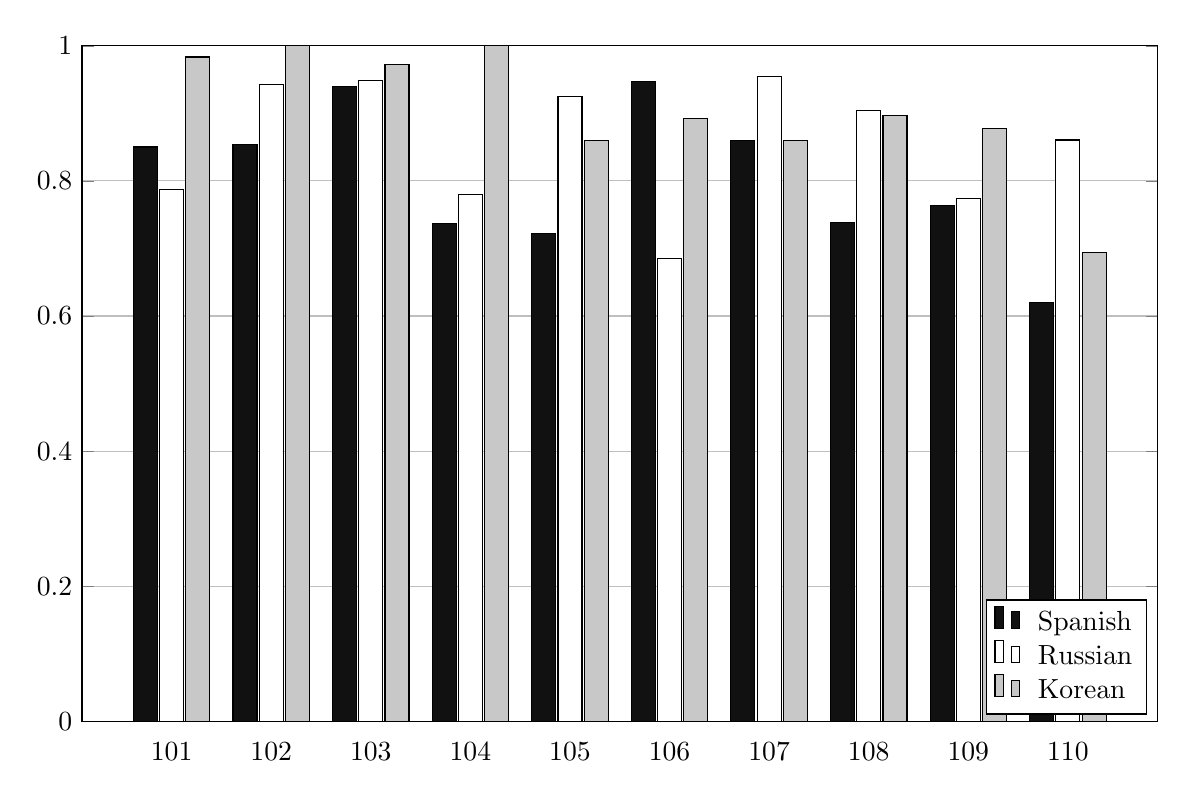
\begin{tikzpicture}
    \begin{axis}[
        width=6in,
	height=4in,
        major x tick style = transparent,
        ybar=2*\pgflinewidth,
        ymajorgrids = true,
        symbolic x coords={101,102,103,104,105,106,107,108,109,110},
        xtick = data,
        scaled y ticks = false,
        enlarge x limits=0.1,
	ymin=0, ymax=1,
        legend cell align=left,
        legend style={
                at={(0.99,0.01)},
                anchor=south east,
                column sep=1ex
        }
    ]
  \addplot[style={bar width=0.12in,fill=bblack,draw=black}]
            coordinates {	(101,0.8502)
				(102,0.8540)
				(103,0.9393)
				(104,0.7372)
				(105,0.7222)
				(106,0.9466)
				(107,0.8596)
				(108,0.7389)
				(109,0.7630)
				(110,0.6205)	    };
%\addplot[style={bar width=0.12in,fill=white,draw=black}]
  \addplot[style={bar width=0.12in,fill=white,every path/.style={postaction={nomorepostaction,pattern=north east lines, pattern color=black}},draw=black}]
            coordinates {	(101,0.7867)
				(102,0.9428)
				(103,0.9492)
				(104,0.7799)
				(105,0.9243)
				(106,0.6850)
				(107,0.9546)
				(108,0.9042)
				(109,0.7736)
				(110,0.8606)	    };
  \addplot[style={bar width=0.12in,fill=wwhite,draw=black}]
            coordinates {	(101,0.9834)
				(102,1.0)
				(103,0.9718)
				(104,1.0)
				(105,0.8596)
				(106,0.8919)
				(107,0.8595)
				(108,0.8967)
				(109,0.8777)
				(110,0.6944)       };
 \legend{Spanish,Russian,Korean}
 \end{axis}
\end{tikzpicture}
\end{document}




